
% Language: english, slovak
% Document type: article (bachelor thesis), report (master thesis)
%%
%% CHECK THE PLACE WITH "!!!!"
%%

%%
%% !!!! select one for BACHELOR THESIS
%%
%\documentclass[a4paper,english,12pt,appendix]{article}
\documentclass[a4paper,slovak,12pt,appendix,twoside,openright,table]{article}

%%
%% !!!! select one for MASTER THESIS
%%
%\documentclass[a4paper,english,12pt,appendix]{report}
%\documentclass[a4paper,slovak,12pt,appendix]{report}

\usepackage{ifthen}
\usepackage{rotating}
\newboolean{english}
\newboolean{bachelor}

%%
%% !!!! for MASTER THESIS set to FALSE
%%
\setboolean{bachelor}{true}

%%
%% !!!! for SLOVAK VERSION set to FALSE
%%
\setboolean{english}{false}



%%
%% Formats and Defs
%%

% Packages
\usepackage{epsf}
\usepackage{epsfig}
\usepackage[T1]{fontenc}
\usepackage{latexsym}
\usepackage{ucs}
\usepackage[utf8x]{inputenc}
\usepackage{float}
\usepackage[usenames]{color}
\usepackage{newcent}
\usepackage{graphicx}
\usepackage{setspace}
\onehalfspacing
\usepackage[numbers]{natbib}
\usepackage{setspace}
\usepackage{url}
\usepackage{eso-pic}
\usepackage{pdfpages}
\usepackage{listings}
\usepackage{verbatim}
\usepackage{moreverb}
\usepackage{microtype}
\usepackage[noauto]{chappg}
\usepackage{lmodern}
\usepackage{appendix}
\usepackage{libertine}
\usepackage{lscape}
\usepackage{amsmath}
\usepackage[table]{xcolor}
\usepackage{tabularx}
\usepackage{pdfpages} 

% Chapter font size
%\usepackage{sectsty}
%\chapternumberfont{\LARGE} 
%\chaptertitlefont{\LARGE}

\usepackage[margin=1in]{geometry}
%Flip odd and even pages margin 
\let\tempmargin\oddsidemargin
\let\oddsidemargin\evensidemargin
\let\evensidemargin\tempmargin
\reversemarginpar
\usepackage{emptypage}
\raggedbottom
\renewcommand{\footnoterule}{\vfill\kern -3pt \hrule width 0.4\columnwidth \kern 2.6pt}

% Language
\ifthenelse {\boolean{english}}
{
	\usepackage[english]{babel}
	
	\renewcommand{\lstlistingname}{Example}
	\renewcommand{\lstlistlistingname}{List of Examples}
}
{
	\usepackage[slovak]{babel}
	\usepackage[IL2]{fontenc}
	
	\renewcommand{\lstlistingname}{Ukážka}
	\renewcommand{\lstlistlistingname}{Zoznam ukážok}	
}

% Section rules
\usepackage{sectsty}
\usepackage{times}

% Bookmarks

% black references
%\usepackage[pdfborder={0 0 0}]{hyperref} 

% red references
\usepackage[colorlinks=true, linkcolor = black, urlcolor = black, citecolor = black, filecolor = black]{hyperref}

% Colors
\definecolor{light-gray}{gray}{0.95}
\definecolor{gray}{gray}{0.2}
\definecolor{blue}{rgb}{0,0,1}
\definecolor{red}{rgb}{1,0,0}
\definecolor{green}{rgb}{0,0.69,0}
\definecolor{yellow}{rgb}{1,0.35,0}

% Listings settings
\lstdefinelanguage{lua}{
	morekeywords={and,break,do,else,elseif,end,false,for,function,if,in,local,nil,not,or,repeat,return,then,true,until,while},
	morekeywords={[2]arg,assert,collectgarbage,dofile,error,_G,getfenv,getmetatable,ipairs,load,loadfile,loadstring,next,pairs,pcall,print,rawequal,rawget,rawset,select,setfenv,setmetatable,tonumber,tostring,type,unpack,_VERSION,xpcall},
	morekeywords={[2]coroutine.create,coroutine.resume,coroutine.running,coroutine.status,coroutine.wrap,coroutine.yield},
	morekeywords={[2]module,require,package.cpath,package.load,package.loaded,package.loaders,package.loadlib,package.path,package.preload,package.seeall},
	morekeywords={[2]string.byte,string.char,string.dump,string.find,string.format,string.gmatch,string.gsub,string.len,string.lower,string.match,string.rep,string.reverse,string.sub,string.upper},
	morekeywords={[2]table.concat,table.insert,table.maxn,table.remove,	table.sort},
	morekeywords={[2]math.abs,math.acos,math.asin,math.atan,math.atan2,math.ceil,math.cos,math.cosh,math.deg,math.exp,math.floor,math.fmod,math.frexp,math.huge,math.ldexp,math.log,math.log10,math.max,math.min,math.modf,math.pi,math.pow,math.rad,math.random,math.randomseed,math.sin,math.sinh,math.sqrt,math.tan,math.tanh},
	morekeywords={[2]io.close,io.flush,io.input,io.lines,io.open,io.output,io.popen,io.read,io.tmpfile,io.type,io.write,file:close,file:flush,file:lines,file:read,file:seek,file:setvbuf,file:write},
	morekeywords={[2]os.clock,os.date,os.difftime,os.execute,os.exit,os.getenv,os.remove,os.rename,os.setlocale,os.time,os.tmpname},
	keywordstyle=\color{blue}\normalfont,
	ndkeywordstyle=\color{black}\normalfont,
	commentstyle=\color{red}\ttfamily,
	stringstyle=\color{green}\ttfamily,
	identifierstyle=\color{gray},
	sensitive=true,
	morecomment=[l]{--},
	morecomment=[s]{--[[}{]]--},
	morestring=[b]",
	morestring=[d]',
	backgroundcolor=\color{white}, 
	frame=single, 
	frameround=ffff,
	captionpos=b,
	basicstyle=\scriptsize
}

\lstdefinelanguage{nil}{
  identifierstyle=\color{gray},
  sensitive=false,
  columns=flexible,
  backgroundcolor=\color{white}, 
  frame=single, 
  frameround=ffff,
  captionpos=b
}

\lstdefinelanguage{javascript}{
  keywords={typeof, new, true, false, catch, function, return, null, catch, switch, var, if, in, while, do, else, case, break},
  ndkeywords={class, export, boolean, throw, implements, import, this},
  sensitive=false,
  comment=[l]{//},
  morecomment=[s]{/*}{*/},
  morestring=[b]',
  morestring=[b]",
  keywordstyle=\color{blue}\normalfont,
	ndkeywordstyle=\color{black}\normalfont,
	commentstyle=\color{red}\ttfamily,
	stringstyle=\color{green}\ttfamily,
	identifierstyle=\color{gray},
	backgroundcolor=\color{white}, 
	frame=single, 
	frameround=ffff,
	captionpos=b,
	basicstyle=\scriptsize
}

\lstdefinestyle{color}
	{identifierstyle=\color{green}\bfseries, commentstyle=\color{yellow}\bfseries, stringstyle=\color{blue}, keywordstyle=\color{red}\bfseries,morecomment=[l]{\#}}

\lstset{postbreak=\small>>\space,prebreak=\small>>,breakindent=13pt,breaklines=true,inputencoding=utf8x,tabsize=2,showtabs=false,tab=$\to$,style=color,basicstyle=\footnotesize\ttfamily\normalfonts,frame=lines,frameround=tttt}

% Figures settings
\usepackage[small,normal,up]{caption2}
\renewcommand{\captionfont}{\small\itshape}
\graphicspath{{figures/}}

%
% this makes list spacing much better.
%
\newenvironment{my_itemize}{
\begin{itemize}
  \setlength{\itemsep}{1pt}
  \setlength{\parskip}{0pt}
  \setlength{\parsep}{0pt}}{
\end{itemize}
}

\newenvironment{my_enumerate}{
\begin{enumerate}
  \setlength{\itemsep}{1pt}
  \setlength{\parskip}{0pt}
  \setlength{\parsep}{0pt}}{
\end{enumerate}
}

\newcommand{\emptyitem}{\item[]}
\newcommand{\myitem}{\item[$-$]}

%Font settings
\makeatletter
\renewcommand{\paragraph}{\@startsection{paragraph}{4}		
{0ex}%
{-3.25ex plus -1ex minus -0.2ex}%
{1.5ex minus 0.2ex}%
 {\normalfont\normalsize\bfseries}}

\makeatother


\stepcounter{secnumdepth}
\stepcounter{tocdepth}

\setcounter{secnumdepth}{3}
\setcounter{tocdepth}{3}


%%%%%%%%%%%%%%%%%%%%%%%%%%%%%%%%%%%%%%%%%%%%%%%%%%%%%%%%%%%%%%%%%%%%%%%%%%%%%%%%%%%%%%%%

%% !!!! set your own definitions

%-------definitions-----
\newcommand{\Author}{Bc. Eva Štalmachová} 
\newcommand{\Title}{RIADENIE NELINEÁRNYCH SPOJITÝCH SYSTÉMOV}
\newcommand{\Supervisor}{Prof. Ing. Ján Murgaš, PhD.}
\newcommand{\Place}{Bratislava }
\newcommand{\Workspace}{Ústav robotiky a kybernetiky}
\newcommand{\Year}{2020}
\newcommand{\Month}{Marec}
\newcommand{\FIIT}{}
\newcommand{\Field}{Kybernetika}
\newcommand{\Program}{Robotika a kybernetika}
\newcommand{\Oponent}{}

%%
%% DON'T TOUCH
%%
%% PDF meta-data 
\hypersetup{%
pdftitle={\Title},%
pdfauthor={\Author},%
pdfkeywords={robot stopar robotika kybernetika},%
}%

%%%%%%%%%%%%%%%%%%%%%%%%%%%%%%%%%%%%%%%%%%%%%%%%%%%%%%%%%%%%%%%%%%%%%%%%%%%%%%%%%%%%%%%%
\hyphenation{ ma-te-ma-tic-ké-ho li-ne-ar-iz-o-va-né li-ne-ar-iz-o-va-nú rov-no-važ-ným poč-ia-toč-né pro-stred-níc-tvom kto-ré-ho ria-diť}
\begin{document}

%%
%% Title Page
%%

\newpage
\begin{center}
\thispagestyle{empty}
\ifthenelse {\boolean{english}}
{
	{\large Slovak University of Technology in Bratislava}\textbf{}\\
	{\Large Faculty of Electrical Engineering and Information Technology}\textbf{}\\[\baselineskip]
}
{
	{\large \textbf{SLOVENSKÁ TECHNICKÁ UNIVERZITA V BRATISLAVE}}\\
	{\large \textbf{FAKULTA ELEKTROTECHNIKY A INFORMATIKY}}\\[\baselineskip]
}
\vspace*{5.5cm}
{\Large \textbf{\Title}}\textbf{}\\
\ifthenelse {\boolean{english}}
{
	\ifthenelse {\boolean{bachelor}}
	{
		{\large Bachelor thesis}\\
	}
	{
		{\large Master thesis}\\
	}
}
{
	\ifthenelse {\boolean{bachelor}}
	{
		{\textbf {TÍMOVÝ PROJEKT}}\\
	}
	{
		{\large Diplomová práca}\\
	}
}
\end{center}
\vspace*{5cm}
\ifthenelse {\boolean{english}}
{
	Study program: \Program\\ 
	Field of Study: \Field\\
	Place: \Place\\
	Vedúci práce: \Supervisor \\\\
}
{
	Študijný program: \hspace*{34.5mm} \Program\\ 
	Študijný odbor: \hspace*{39mm} \Field\\
	Školiace pracovisko: \hspace*{30mm} \Workspace\\
	Vedúci projektu: \hspace*{37.5mm} \Supervisor \\\\\\\\\\
}
\large \textbf{\Place \Year} \hspace*{6.5cm} \large \textbf{\Author}\\
\hspace*{10cm} \large \textbf{Bc. Marek Trebuľa}\\
\hspace*{10.0cm} \large \textbf{Bc. Denis Vasko}\\
\hspace*{10cm} \large \textbf{Bc. Ján Urdianyk}

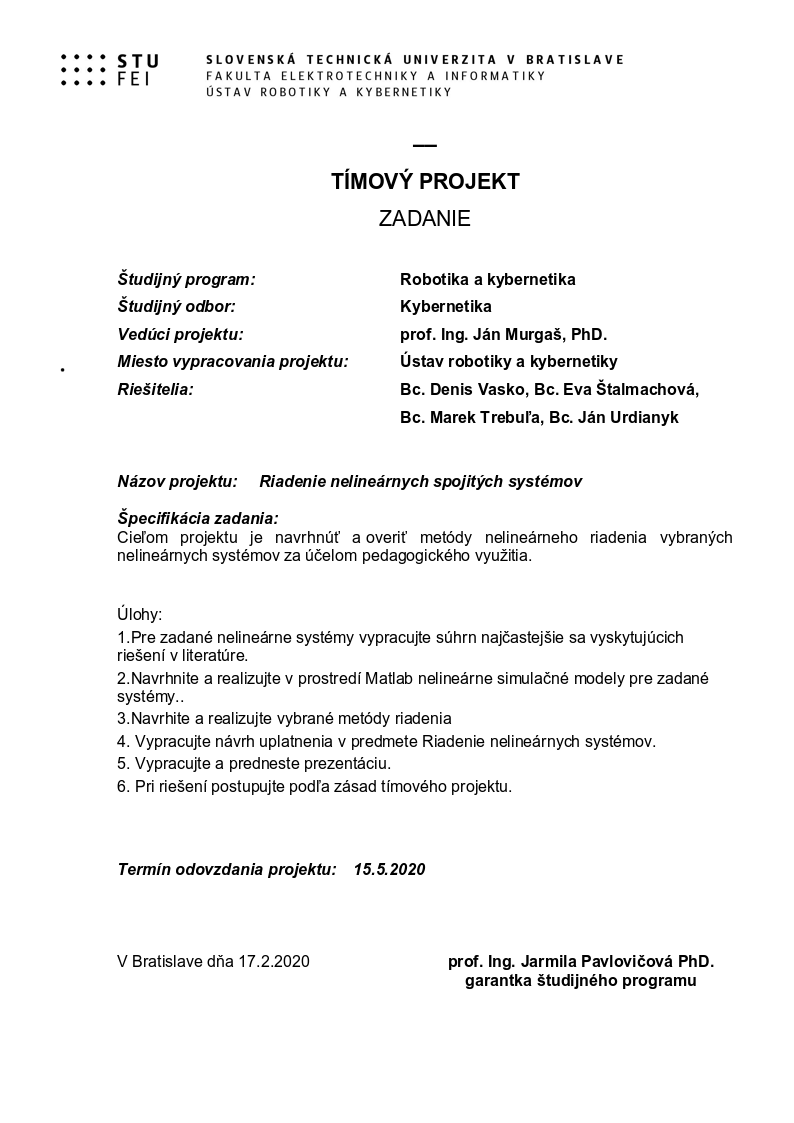
\includepdf[pages=1]{TP_zadanie_1_KYB.png}
%%
%% Anotation
%%

% Arabske cislovanie dov hlavnej prace
%\pagenumbering{roman}\setcounter{page}{2}
%\newpage
\thispagestyle{plain}
\noindent


%%
%% Declaration
%%
%\newpage
\thispagestyle{plain}
\vspace*{15cm} 
\begin{large}
\noindent
%\textbf{ACKNOWLEDGMENTS} \\
\textbf{POĎAKOVANIE} \\
\end{large}
\noindent
Lorem ipsum dolor sit amet, consectetur adipisicing elit, sed do eiusmod tempor incididunt ut labore et dolore magna aliqua. Ut enim ad minim veniam, quis nostrud exercitation ullamco laboris nisi ut aliquip ex ea commodo consequat.....
\newpage
\thispagestyle{plain}
\vspace*{15cm} 
\begin{large}
\noindent
%\textbf{Čestné prehlásenie} \\
\textbf{ČESTNÉ PREHLÁSENIE} \\
\end{large}
\noindent
Lorem ipsum dolor sit amet, consectetur adipisicing elit, sed do eiusmod tempor incididunt ut labore et dolore magna aliqua....\\
\vspace*{0.5cm}\\
\hspace*{10cm}............................\\
\hspace*{10.7cm} \Author

%%
%% Contents
%%
%\pagestyle{empty}
\newpage
\tableofcontents{}
\setcounter{secnumdepth}{0}
\newpage
\section{Zoznam použitých skratiek}

 
\setcounter{secnumdepth}{1}
%%
%% Lists
%%
% \newpage
% List of Figures
% \listoffigures  
% \newpage
% List of Tables
% \listoftables
% \newpage
% List of Listings
% \lstlistoflistings


%%
%% Clear Page And Set New Page Counter
%%
% Klasicke cislova, ked zapnes rimske zapni aj toto 
%\clearpage
%\pagenumbering{arabic}
%\setcounter{page}{1}

\ifthenelse {\boolean{bachelor}}
{
	\sectionfont{\sectionrule{0pt}{0pt}{-2ex}{0.5pt}}
}
{
	\sectionfont{\sectionrule{0pt}{0pt}{-2ex}{0pt}}
}
%\thispagestyle{empty}%
%\addtocounter{page}{-1}%
%\newpage
%%
%% Introduction
%%
\newpage
\ifthenelse {\boolean{bachelor}}
{
	%\section{Introduction}
	\section{Úvod}
}
{
	%\chapter{Introduction}
%	\chapter{Úvod}
}

    V tímovom projekte sa venujeme definovaniu niekoľkých modelov systémov v stavovom opise, vhodných na demonštráciu návrhu nelineárneho riadenia pomocou metód vstupno-stavovej a vstupno-výstupnej linearizácie a návrhom nelineárneho riadenia pre dané modely. Navrhnuté nelineárne riadenie porovnávame s lineárnym PID regulátorom a uvádzame aj základné matematické princípy, využívané pri návrhu pomocou uvedených metód.

    V časti \ref{sec:matematicke_zaklady} sa venujeme niektorým matematickým princípom, ktorých znalosť je nevyhnutná pre pochopenie metód, ale aj ďalšieho textu, v celom rozsahu. Konkrétne táto časť zahŕňa opakovanie k nasledujúcim témam: stavový opis systému, rovnovažné stavy a linearizácia. 
    
    Časť \ref{sec:vsl} sa zaoberá návrhom nelineárneho riadenia pomocou metódy vstupno-stavovej linearizácie. Sú tu prezentované dva príklady, ku každému je vypracovaný návrh riadenia danou metódou a pre porovnanie je navrhnutý aj PID regulátor pre linearizáciu systému v rovnovažnom stave.

    Návrhu pomocou metódy vstupno-výstupnej linearizácie sa venujeme v časti \ref{sec:vvl}. Podobne ako v predchádzajúcej časti, aj tu sa venujeme okrem návrhu pomocou hlavnej metódy aj návrhu PID regulátora pre linearizovaný systém.

    V časti \ref{sec:integracia} stručne opíšeme spôsoby ako by sa daný materiál dal integrovať do predmetu Riadenie Nelineárnych Systémov.

    V časti \ref{sec:riadproj} sa venujeme predstaveniu riešiteľského kolektívu, plánu projektu, dohodnutým metódam práce a záznamom o stretnutí. 

    Príkladáme aj program písaný v matlabe, spolu s manuálom na použitie, vhodný na ukážku navrhnutých zákonov riadenia pre jednoduchý príklad riadenia polohy matematického kyvadla. V programe sú implementované nelineárne zákony riadenia a aj dva PID regulátory navrhnuté pre linearizáciu kyvadla v stabilnom a v nestabilnom rovnovažnom stave. 




%%
%% analysis
%%
\newpage
\ifthenelse {\boolean{bachelor}}
{
	\section{Matematické základy}\label{sec:matematicke_zaklady}
	\subfile{matzaklady/matzaklady}

    \newpage
    \clearpage 
	\section{Spätnoväzbová linearizácia - vstupno-stavová}\label{sec:vsl}
 	\subfile{vsPr1/vsPr1.tex}
 	\subfile{vsPr2/svlvvPr2.tex}

    \newpage
    \clearpage 
	\section{Spätnoväzbová linearizácia - vstupno-výstupná}\label{sec:vvl}
 	\subfile{svlvvPr1/svlvvPr1}
 	\subfile{svlvvPr2_marek/svlvvPr2.tex}

    \newpage
    \clearpage 
    \section{Integrácia do predmetu RNS}\label{sec:integracia}
 	\subfile{integracia/integracia.tex}
}
{
	%\chapter{Analysis}
%	\chapter{Analyza}
}


% Tu začíname doplnat text. Ked chcete skompilovat ctrl+s a skomplilujete main.tex nekompilujte tento subor. Také zakladné pravidlá aby sme sa vedeli orientovať obrázky davajte do priečinka figures. Ak budete chciet robit referenciu na obrazok, rovnicu alebo sekcie : \ref{sec:matematicke_zaklady}. Preto prosím každý obrázok, sekciu a rovnicu label-ujte, ulahci to robotu. Ja mam vo zvyku sekcie nazyvat sec:nazov, obrazky fig:nazov, rovnice eq:nazov. \cite{slotine1991applied}
% 
% \newpage
% \section{Metóda spätnoväzobnej linearizácie}
% tu by mohla byt nejaka teoria o spätnoväzobnej linearizácií
% \newpage
% \section{Vstupno-stavová metóda spätnoväzobnej linearizácie}
% tu by mohla byt nejaka teoria o spätnoväzobnej linearizácií VS
% \subsection{Návrh riadenia - Príklad 1.}
% tu bude priklad 1 + vypocet
% \subsection{Simulačná schéma - Príklad 1.}
% tu schema 
% \subsection{Overenie navrhnutého riadenia - Príklad 1.}
% tu vysledky co sme dosiahli plus nejaky pokec k tomu
% \subsection{Návrh riadenia - Príklad 2.}
% \subsection{Simulačná schéma - Príklad 2.}
% \subsection{Overenie navrhnutého riadenia - Príklad 2.}
% \subsection{Porovnanie navrhnutého riadenia s lineárnym regulátorom}
% 
% \newpage
% \section{Vstupno-výstupná metóda spätnoväzobnej linearizácie}
% 	\subfile{svlvvPr1/svlvvPr1}
% 
% \subsection{Príklad s internou dynamikou}
% 
% 
% \subsection{Simulačná schéma - Príklad 1.}
% \subsection{Overenie navrhnutého riadenia - Príklad 1.}
% \subsection{Návrh riadenia - Príklad 2.}
% \subsection{Simulačná schéma - Príklad 2.}
% \subsection{Overenie navrhnutého riadenia - Príklad 2.}
% \subsection{Porovnanie navrhnutého riadenia s lineárnym regulátorom}
% 
% 
% 
% \newpage
% \section{Prehlad takych zakladnych latex veci - Tato sekcia tu nebude }\label{sec:prehlad}
% 
% $ H = \begin{bmatrix} 18.9000 & 47.6000 & 63.0000 \\ 28.7000 & 44.1000 & 45.5000 \\ 15.4000  & 16.8000  & 12.6000 \\ 1.4000 & -2.8000  & -7.0000 \end{bmatrix}$
% $ y = \begin{bmatrix} -64.4000 \\ -41.3000 \\ -8.4000 \\ 8.4000 \end{bmatrix}$
% 
% \begin{equation}\label{eq:Rovnica}
% F(s) = \frac{K}{1+Ts}e^{-Ds}
% \end{equation}
% 
% 
% \textbf{Neznáme parametre:} $K,T,D$
% 
% 
% \textbf{Postup:}
% \begin{enumerate}
% \item \[K = y(\infty); K = 3.8059\]
% \item \[T = \frac{t_2-t_1}{ln(\frac{K-y_1}{K-y_2})} ; T = 0.4452 \]
% \item \[x = \frac{ln(\frac{K-y_1}{K})}{ln\frac{K-y_2}{K}}, D = \frac{t_2x-t_1}{x-1}; x = 0.2093, D = 0.0857\]
% \end{enumerate}
% 
% \textbf{Postup:}
% \begin{itemize}
% \item \[K = y(\infty); K = 3.8059\]
% \item \[T = \frac{t_2-t_1}{ln(\frac{K-y_1}{K-y_2})} ; T = 0.4452 \]
% \item \[x = \frac{ln(\frac{K-y_1}{K})}{ln\frac{K-y_2}{K}}, D = \frac{t_2x-t_1}{x-1}; x = 0.2093, D = 0.0857\]
% \end{itemize}
% 
% \begin{table}[h!]
% \centering
%  \begin{tabular}{|c | c | c | c | c|} 
%  \hline
%  $k$ & $\theta_{k}^{*}$ & $P_{k}$ & $e_{k}$ &  $Q_{k}$ \\ [0.5ex] 
%  \hline\hline
%  0 & $ \begin{bmatrix} 0 \\ 0 \\ 0 \end{bmatrix}$ & $ 10^{10} *\begin{bmatrix}  1 & 0 & 0 \\ 0 & 1 & 0 \\ 0 & 0  & 1 \end{bmatrix}$ & 0 & 0 \\ 
%  \hline
%  1 & $ \begin{bmatrix} -0.1846 \\ -0.4650 \\ -0.6155 \end{bmatrix}$ & $ 10^{9} *\begin{bmatrix}  9.4581 & -1.3648 & -1.8063 \\ -1.3648 & 6.5628 & -4.5492 \\ -1.8063  & -4.5492  & 3.9790 \end{bmatrix}$ & -64.4000 & $6.2915*10^{-11}$ \\ 
%  \hline
%  2 & $ \begin{bmatrix} 0.4987 \\ -0.2360 \\ -0.9935 \end{bmatrix}$ & $ 10^{9} *\begin{bmatrix}  2.4082 & -3.7279 & 2.0942 \\ -3.7279 & 5.7707 & -3.2418 \\ 2.0942 & -3.2418  & 1.8211 \end{bmatrix}$ & 12.5111 & $1.2915*10^{-10}$ \\ 
%  \hline
%  3 & $ \begin{bmatrix} 1.6486 \\ -2.0160\\ 0.0064 \end{bmatrix}$ & $\begin{bmatrix}  13.6362 & -21.4003 & 12.0936 \\ -21.4002 & 33.5946 & -18.9875 \\ 12.0935 & -18.9874  & 10.7325 \end{bmatrix}$ & 0.4031 & $6.7820*10^{-10}$ \\ 
%   \hline
%  4 & $ \begin{bmatrix} 0.8406 \\ -0.7436 \\ -0.7140 \end{bmatrix}$ & $\begin{bmatrix}  4.3694 & -6.8073 & 3.8314 \\ -6.8066 & 10.6133 & -5.9761 \\ 3.8311 & -5.9762  & 3.3659 \end{bmatrix}$ & 0.4920 & 0.0704 \\ [1ex] 
% 
%  \hline
%  \end{tabular}
% \end{table}
% 
% \begin{figure}[H]
% \begin{center}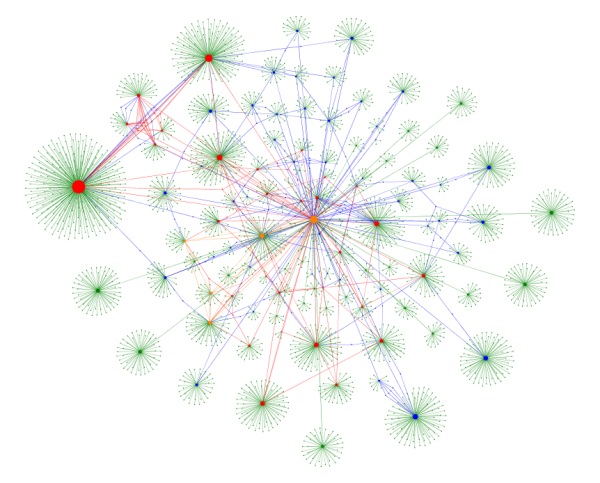
\includegraphics[scale=0.48]{figure.png}\end{center}
% \caption{Name figure}\label{fig:figure}
% \end{figure}
% \subsection{Enumeration}
% %\subsection{Číslovaný zoznam}
% \begin{my_enumerate}
% 	\item {goal 1}
% 	\begin{my_enumerate}
% 		\item {goal 1.a}
% 		\item {goal 1.b}
% 	\end{my_enumerate}
% 	\item {goal 2}
% 	\item {goal 3}
% \end{my_enumerate}
% \subsection{Itemization}
% %\subsection{Zoznam}
% \begin{my_itemize}
% 	\item {item 1}
% 	\begin{my_itemize}
% 		\item {item 1.1}
% 		\item {item 1.2}
% 	\end{my_itemize}
% 	\item {item 2}
% 	\item {item 3}
% \end{my_itemize}




%%
%% design
%%
%\newpage
\ifthenelse {\boolean{bachelor}}
{
	%\section{Design}
	\section{Návrh}
}
{
	%\chapter{Design}
	\chapter{Návrh}
}
Lorem ipsum dolor sit amet, consectetuer adipiscing elit, sed diam nonummy nibh euismod tincidunt ut laoreet dolore magna aliquam erat volutpat. Ut wisi enim ad minim veniam, quis nostrud exerci tation ullamcorper suscipit lobortis nisl ut aliquip ex ea commodo consequat. 
\ifthenelse {\boolean{bachelor}}
{
	%\subsection{Subsection}
	\subsection{Podčasť}
}
{
	%\section{Subsection}
	\section{Podčasť}
}
\label{label}
Lorem ipsum dolor sit amet, consectetuer adipiscing elit, sed diam nonummy nibh euismod tincidunt ut laoreet dolore magna aliquam erat volutpat. Ut wisi enim ad minim veniam, quis nostrud exerci tation ullamcorper suscipit lobortis nisl ut aliquip ex ea commodo consequat. Duis autem vel eum iriure dolor in hendrerit in vulputate velit esse molestie consequat, vel illum dolore eu feugiat nulla facilisis at vero eros et accumsan et iusto odio dignissim qui blandit praesent luptatum zzril delenit augue duis dolore te feugait nulla facilisi. Nam liber tempor cum soluta nobis eleifend option congue nihil imperdiet doming id quod mazim placerat facer possim assum. Typi non habent claritatem insitam; est usus legentis in iis qui facit eorum claritatem. Investigationes demonstraverunt lectores legere me lius quod ii legunt saepius. Claritas est etiam processus dynamicus, qui sequitur mutationem consuetudium lectorum. Mirum est notare quam littera gothica, quam nunc putamus parum claram, anteposuerit litterarum formas humanitatis per seacula quarta decima et quinta decima. Eodem modo typi, qui nunc nobis videntur parum clari, fiant sollemnes in futurum.

%%
%% test
%%
%\newpage
\ifthenelse {\boolean{bachelor}}
{
	%\section{Results}
	\section{Výsledky}
}
{
	%\chapter{Results}
	\chapter{Výsledky}
}
Lorem ipsum dolor sit amet, consectetuer adipiscing elit, sed diam nonummy nibh euismod tincidunt ut laoreet dolore magna aliquam erat volutpat. Ut wisi enim ad minim veniam, quis nostrud exerci tation ullamcorper suscipit lobortis nisl ut aliquip ex ea commodo consequat. 

\ifthenelse {\boolean{bachelor}}
{
	%\subsection{Subsection}
	\subsection{Podčasť}
}
{
	%\section{Subsection}
	\section{Podčasť}
} 
\label{label}
Lorem ipsum dolor sit amet, consectetuer adipiscing elit, sed diam nonummy nibh euismod tincidunt ut laoreet dolore magna aliquam erat volutpat. Ut wisi enim ad minim veniam, quis nostrud exerci tation ullamcorper suscipit lobortis nisl ut aliquip ex ea commodo consequat. Duis autem vel eum iriure dolor in hendrerit in vulputate velit esse molestie consequat, vel illum dolore eu feugiat nulla facilisis at vero eros et accumsan et iusto odio dignissim qui blandit praesent luptatum zzril delenit augue duis dolore te feugait nulla facilisi. Nam liber tempor cum soluta nobis eleifend option congue nihil imperdiet doming id quod mazim placerat facer possim assum. Typi non habent claritatem insitam; est usus legentis in iis qui facit eorum claritatem. Investigationes demonstraverunt lectores legere me lius quod ii legunt saepius. Claritas est etiam processus dynamicus, qui sequitur mutationem consuetudium lectorum. Mirum est notare quam littera gothica, quam nunc putamus parum claram, anteposuerit litterarum formas humanitatis per seacula quarta decima et quinta decima. Eodem modo typi, qui nunc nobis videntur parum clari, fiant sollemnes in futurum.

%%
%% Conclusion
%%
\newpage
\ifthenelse {\boolean{bachelor}}
{
	%\section{Conslusions}
	\section{Záver}
}
%{
	%\chapter{Conclusions}
%	\chapter{Záver}
%}



%%
%% References
%%
\newpage
\addcontentsline{toc}{section}{\refname}
%\bibliography{references}
\bibliographystyle{plainnat}

\begin{thebibliography}{9}
\bibitem{slotine1991applied} SLOTINE, Jean-Jacques E., et al. Applied nonlinear control. Englewood Cliffs, NJ: Prentice hall, 1991.
\end{thebibliography}
%%
%% Appendix
%%
%\ifthenelse {\boolean{bachelor}}
%{
%}
%{
%	\ifthenelse {\boolean{english}}
%	{
%		\renewcommand{\appendixname}{Appendix}
%		\renewcommand{\appendixtocname}{Appendix}
%	}
%	{
%		\renewcommand{\appendixname}{Príloha}
%		\renewcommand{\appendixtocname}{Prílohy}
%	}
%	\pagenumbering{bychapter}
%}
\appendix
\newpage
\thispagestyle{plain}


\end{document}

%%%%%%%%%%%%%%%%%%%%%%%%%%%%%%%%%%%%%%%%%%%%%%%%%%%%%%%%%%%%%%%%%%%%%%%%%%%%%%%%%%%%%%%%

%%
%% !!!! set your own details
%%
\begin{comment}
[x] [], [Tímový projekt]
\end{comment}
